\seccion{Entropias y divergencias generalizadas}
\label{sec:SZ:Generalizadas}

A pesar de que la entropia de Shannon y sus cantidades asociadas demostraron sus
potencias tan de un punto de vista descriptivo que en termino de aplicaciones en
la  transmisi\'on  de  la  informaci\'on  y  la  compresi\'on,  varios  nociones
informacionales, de  tipo entropias o  divergencias, aparecieron luego.  En esta
secci\'on no se  desarollar\'a todos los enfoques ni  todas las aplicaciones tan
la  literatura es  importante. La  meta  es dar  los caminos  conduciendo a  las
generalizaciones de la  entropia de Shannon por un lado, y  de la divergencia de
Kullback-Leibler por el otro lado. No son siempre vinculados, a pesar de que sea
desirable que a cada entropia sean asociados nociones de entropias condicionales
y relativas.

% ================================= Salicru

\subseccion{Entropias y propiedades}
\label{sec:SZ:Salicru}

Si  la entropia  de  Shannon  fue el  punto  de salida  fundamental  en todo  el
desarollo de la teoria de la informaci\'on, un poco mas de una decada despues de
su    papel   clave    y   muy    completo,   R\'enyi    propuso    una   medida
generalizada~\cite{Ren61}. Su  punto de  vista fue mas  matematico que  fisico o
ingeniero.  Retom\'o los axiomas de Fadeev~\cite{Fad56, Fad58, Khi57}
% Feinstein, cf ref  de R��nyi
%
a  probabilidades  incompletas   $p  =  \begin{bmatrix}  p_1  &   \cdots  &  p_n
\end{bmatrix}^t,  \quad p_i  \ge  0,  \quad w_p  =  \sum_i p_i  \le  1$: (i)  la
invarianza de  $H(p)$ por permutaci\'on de  os $p_i$, (ii) la  continuidad de la
incerteza elemental  $H(p_i)$ ($p_i$ visto como  probabilidad incompleta), (iii)
$H\left( \frac12 \right) = 1 $,  (iv) la aditividad $H(p \otimes q) = H(p)+H(q)$
donde $p \otimes q$ es el producto de Kronecker~\footref{foot:SZ:Kronecker},
%\footnote{$\begin{bmatrix} p_1 &
%\cdots & p_n \end{bmatrix}^t \otimes \begin{bmatrix} q_1 & \cdots & q_m
%\end{bmatrix}^t = \begin{bmatrix} p_1 q_1 & \cdots  & p_1 q_m & \cdots & p_n q_1
%&  \cdots  &  p_n  q_m  \end{bmatrix}^t$.}, 
\ie  probabilidad conjunta  de dos  variables independientes,  y  consider\'o en
lugar de la recursividad un axioma  dicho de valor promedio, axioma muy parecido
a la recursividad. Para $p$ \ y \ $q$ probabilidades incompletas tales que $p \,
\cup  \,  q   =  \begin{bmatrix}  p_1  &   \cdots  &  p_n  &  q_1   &  \cdots  &
  q_m \end{bmatrix}^t$ sea incompleta ($w_p + w_q \le 1$), el axioma (v) es $H(p
\, \cup \,  q) = \frac{w_p \, H(p)  + w_q \, H(q)}{w_p +  w_q}$.  Demostr\'o que
con (v) en lugar  de la recursividad, el conjunto de axiomas  conduce de nuevo a
la  entropia de  Shannon.   La  generalizaci\'on propuesta  por  R\'enyi era  de
generalizar  el axioma  (v)  remplazando  la media  aritm\'etico  por una  media
generalizada (v')  $H^\ren(p \, \cup \,  q) = g^{-1} \left(  \frac{w_p \, g\big(
    H^\ren(p) \big) + w_q \,  g\big( H^\ren(q) \big)}{w_p + w_q}\right)$ con $g$
estrictamente  monotona y  continua,  llamado media  {\it cuasi-aritm\'etica,  o
  quasi-lineal,  o  de  Kolmogorov-Nagumo}.   De  las propiedades  de  la  media
cuasi-aritmetica~\cite{Nag30,  Kol30,  Kol91, HarLit52},  eso  es equivalente  a
buscar una  entropia elemental $H^\ren(p_i)$  y remplazar la  media aritm\'etica
$\sum_i  p_i H^\ren(p_i)$  por una  media de  Kolmogorov-Nagumo,  $g^{-1} \left(
  \sum_i p_i g\big( H^\ren(p_i)  \big) \right)$.  R\'enyi propus\'o la funci\'on
de Kolmogorov-Nagumo $g_\beta(x) = 2^{(\beta-1)  x}, \quad \beta >0, \quad \beta
\ne 1$,  probando que  la entropia que  los axiomas  (i)-(ii)-(iii)-(iv)-(v') se
cumplen y conduce a la entropia de R\'enyi de un vector de probabilidad $p$,
%
\[
H_\beta^\ren(p) = \frac{1}{1-\beta} \log_2 \left( \sum_{i=1}^n p_i^\beta \right)
\]
%
\noindent   Relaxando  el  axioma   (iii),  se   puede  elegir   $g_\beta(x)  =
a^{(\beta-1) x}, \quad  a > 0, \quad a  \ne 1$; el logaritmo ser\'a  de la base
$a$ cualquiera; En  lo que sigue, usaremog $\log$ sin  precisar la elecci\'on de
base.   R\'enyi  nombr\'o  esta  medida  de incerteza  {\it  entropia  de  orden
$\beta$}. Notablemente,
%
\[
H_1^\ren(p)  \equiv   \lim_{\beta  \to   1}  H_\beta^\ren(p)   =   H(p)  \quad
\mbox{entropia de Shannon}
\]
% \noindent En otros terminos, la clase de R\'enyi contiene como caso particular
la  entropia  de  Shannon.  En  su  papel,  R\'enyi  introdujo una  ganancia  de
informaci\'on,  parecida  a  una  entropia  relativa,  probando  que  las  solas
entropias admisibles  son la  de Shannon  y la que  introdujo. Volveremos  en la
secci\'on siguiente sobre esta entropia  relativa, o divergencia de R\'enyi. Por
axiomas,     las     propiedades    \ref{prop:SZ:continuidad}     (continuidad),
\ref{prop:SZ:permutacion}       (invarianza      por       permutaci\'on)      y
\ref{prop:SZ:aditividad} (additividad)  de la  entropia de Shannon  se conservan
entonces  en  el  marco   de  R\'enyi  y  se  pierde  \ref{prop:SZ:recursividad}
(recursividad), todav\'ia por axiomas. Veremos luego la otras que se conservan o
modifican en un marco mas general.

Unos  a\~nos despu\'es de  R\'enyi, de  la famosa  escuela matematica  checa, J.
Havrda   \&    F.    Charv\'at   en~\cite{HavCha67}    (ver   tambi\'en~\cite[en
checo]{Vaj68}) volvieron a los axiomas de Khintchin, para extender la entopia de
Shannon,  \ie  considerando  (i)   la  invarianza  por  permutaci\'on,  (ii)  la
continuidad, (iii) la expensividad, (iv) $H^\hc(1) = 0$ y $H^\hc\left( \frac12 ,
  \frac12   \right)  =   1$,  pero   generalisando  la   recursividad   por  (v)
$H^\hc(p_1,\ldots,p_n)    =   H^\hc(p_1,\ldots,p_{n-2},p_{n-1}+p_n)    +   \beta
(p_{n-1}+p_n)^\beta H^\hc\left( \frac{p_{n-1}}{p_{n-1} + p_p},\frac{p_n}{p_{n-1}
    + p_p}  \right), \quad  \beta > 0$~\footnote{En  sus papel, lo  imponen para
  cualquier pars $p_i, p_j$ sin imponer la invarianza por permutaci\'on, pero es
  equivalente a la  exposici\'on de este parafo.}.  Con $\beta  = 1$ se recupera
la  recursividad estandar,  pero  con $\beta  \ne  1$ eso  permite  dar un  peso
diferente a la incerteza del estado interno \ie probabilidades que se juntan (la
describen como clasificaci\'on refinada).  Estos axiomas conducen necesariamente
a la entropia (teorema~1)
%
\[
H_\beta^\hc(p) = \frac{1}{1-2^{1-\beta}} \left( 1 - \sum_i p_i^\beta \right)
\]
%
que nombraron {\it $\beta$-entropia structural}.  De nuevo, relaxando el axioma
(iv),  se puede  remplazar en  el coeficient  $2^{1-\beta}$  por $a^{1-\beta},
\quad a >  0, \quad a \ne 1$. De  nuevo, parae que la entropia  de Shannon es un
caso particular,
%
\[
H_1^\hc(p)  \equiv   \lim_{\beta  \to   1}  H_\beta^\hc(p)   =   H(p)  \quad
\mbox{entropia de Shannon}
\]
% Por   axioma,   se   conservan   las   propiedades   \ref{prop:SZ:continuidad}
(continuidad), \ref{prop:SZ:expansabilidad} (expansabilidad)  de Shannon en este
marco. Se  prob\'o tambi\'en  que se conserva  la propiedad de  concavavidad con
respeto    a   los   $p_i$    \ref{prop:SZ:concavidad},   la    de   maximalidad
\ref{prop:SZ:cotamaxima}    alcanzada   para    una    distribuci\'on   uniforma
(teorema~2). Aun  que no aparece  as\'i en el  papel, satisface la  propiedad de
Schur-concavidad  \ref{prop:SZ:Schurconcavidad}  (teorema~3).  A  pesar  de  que
mencionan que $H_\beta^\hc$ sea  diferente que $H_\beta^\ren$, es sencillo ver
que hay  un mapa  uno-uno entre  las dos entropias.  Se notara  en un  marco mas
general otras propiedades.

Independiente  de Havrda  \&  Charv\'at, todav\'ia  en  el este,  en la  escuela
h\'ugara, Z.  Dar\'oczy en~\cite{Dar70} defino la entropia $H^f$ a partir de una
{\it  funci\'on  informaci\'on}  $f$   satifaciendo  (i)  $f(0)  =  f(1)$,  (ii)
$f\left(\frac12\right)  = 1$  \ y  la ecuaci\'on  funcional (ii)  $f(x)  + (1-x)
f\left(  \frac{y}{1-x} \right)  = f(y)  + (1-y)  f\left(  \frac{x}{1-y} \right)$
sobre  $\{  (x,y)  \in [0  ;  1)^2,  \quad  x+y  \le  1 \}$,  siendo  $H^f(p)  =
\sum_{i=2}^n s_i  f\left( \frac{p_i}{s_i} \right), \quad  s_i = \sum_{j=1}^{i-1}
p_j$.   Dar\'oczy mostr\'o  que  si $f$  es medible,  o  continua en  $0$, o  no
negatiba  y  acotada, necesariamente  $f(x)  =  h_2(x) =  -x  \log_2  x -  (1-x)
\log_2(1-x)$,   conduciendo   a  la   entropia   de   Shannon  (teorema~1;   ver
tambi\'en~\cite{Lee64,  Tve58, Ken64}).   En otros  terminos, su  axioma  (v) es
alternativa a  la recursividad.  Para  extender la entropia de  Shannon, propuso
extender este axioma  (v) por la ecuaci\'on funcional  $f_\beta(x) + (1-x)^\beta
f_\beta\left(  \frac{y}{1-x} \right)  = f_\beta(y)  +  (1-y)^\beta f_\beta\left(
  \frac{x}{1-y}  \right)$,   lo  que   condujo  necesariamente  a   la  entropia
(teoremas~2 y~3)
%
\[
H_\beta^\dar(p) = \frac{1}{1-2^{1-\beta}} \left( 1 - \sum_i p_i^\beta \right)
\]
%
\noindent  es  decir  nada  mas  que  la  entropia  introducida  por  Havdra  \&
Charv\'at. En lo que sigue, se la denota $H_\beta^\hcd$. Sin embargo, el estudio
de Dar\'oczy fue  mas intensivo que el de Havdra  \& Charv\'at.  Primero, not\'o
el mapa  entre su  entropia y la  de R\'enyi. Adicionalmente  a Havdra-Charv\'at
probaron que se conserva  la propiedad \ref{prop:SZ:permutacion} (invarianza por
permutaci\'on, que no era un  axioma en su enfoque), $H_\beta^\hcd\left( \frac12
  ,  \frac12   \right)  =  1$   (lo  llama  normalizaci\'on),   la  expansividad
\ref{prop:SZ:expansabilidad},   una  additividad  extendida,   una  recursividad
extendida  precisamente  del modelo  de  Havrda-Charv\'at (teorema~4).   Prob\'o
tambi\'en   \ref{prop:SZ:positividad},   positividad   alcanzado  en   el   caso
deterministico y  la m\'aximalidad \ref{prop:SZ:cotamaxima} en  el caso uniforme
(teorema~6),  que incidentalmente  $H_\beta^\hcd\left( \frac1\alpha  ,  \ldots ,
  \frac1\alpha \right)$ crece con el  cardinal $|\X| = \alpha$.  Muy interesante
tambi\'en es se puede definir una entropia condicional en el mismo modelo que en
el caso de Shannon $H_\beta^\hcd(X|Y) = \sum_y \left[ p_{X|Y}(x,y) \right]^\beta
H_\beta^\hcd(   p_{X|Y}(\cdot,y)   )$,   que   existe  una   regla   de   cadena
\ref{prop:SZ:cadena}, $H_\beta^\hcd(X,Y)  = H_\beta^\hcd(Y) + H_\beta^\hcd(X|Y)$
y    que    \ref{prop:SZ:condicionar}    condicionar    reduce    la    entropia
$H_\beta^\hcd(X|Y) \le H_\beta^\hcd(X)$  (teorema~8).  Mostr\'o tambi\'en que si
se pierde  la additividad, se  obiene para \  $X$ \ e  \ $Y$ \  independientes \
$H_\beta^\hcd(X,Y) = H_\beta^\hcd(X) +  H_\beta^\hcd(Y) + \left( 2^{1-\beta} - 1
\right) H_\beta^\hcd(X) H_\beta^\hcd(Y)$.  La  propiedades de regla de cadena le
permiti\'o  revisitar  la  caracterisaci\'on  de  un canal  de  transmisi\'on  y
redefinir una capacidad canal extendidas (capacidad tipo $\beta$; basicamente se
usa el  mismo enfoque que Shannon,  pero usando $H_\beta^\hcd$ en  lugar de $H$,
ver secci\'on~6 del papel).

Estas  entropia fueron (re)descubiertos  varios otras  veces y/o  estudiados mas
detenidamente    en    varios     campos    y    varios    extensiones    fueron
introducidas~\cite[entre  otros]{Var66, Oni66,  Kap67,  Vaj68, LinNie71,  Ari71,
Bur72, AczDar75,  ShaMit75, ShaMit75,  ShaTan75, Mit75, BoeLub80,  Fer80, Tsa88,
Rat91, Kan01}.   Un primer enfoque  mas general es  debido a S.  Arimoto  en los
primeros a\~nos de  la decada 1970~\cite{Ari71} y rediscubierto  y estudiado con
mas  detaller y  una decada  despues por  Burbea y  Rao~\cite{BurRao82}  y luego
estudiado   por   Salicr\'u~\cite{Sal87}.     La   medida   propuesta,   llamada
$\phi$-entropia, es definida por
%
\[
\hphi{p} = -\sum_i \phi(p_i) \qquad \mbox{con} \qquad \phi \: \mbox{ convexa}
\]
%
Burbea  y  Rao  asociaron  una  medida  de  divegencia  a  esta  entropia.   Las
$\phi$-entropias contienen Shannon como caso  particular ($\phi(x) = x \log x$),
as\'i  que  la  clase   de  Havdra-Charv\'at-Dar\'oczy  ($\phi(x)  =  \frac{x  -
  x^\beta}{2^{1-\beta}-1}$)  como mencionado, pero  no la  clase de  R\'enyi. De
hecho, las $\phi$-entropias se enmarcan en una clase un poco mas amplia, llamada
$(h,\phi)$-entropias~\cite{SalMen93, MenMor97}. Cambiamos ac\`a substancialmente
su escritura por razones homogeneidad con la $\phi$-entropia (y las divergencias
que se introducira luego)~\footnote{En la literatura, no hay el signo $-$, y hay
  que invertir concava y convexa.}
%
\begin{definicion}[$(h,\phi)$-entropia]
La $(h,\phi)$-entropia de una  distribuci\'on de probabilidad $p_X$ definida sobre
$\X$ de cardinal finito $|\X| = \alpha$ es definida por
%
\[
\hhphi{X}  = \hhphi{p_X}  = h\left(  - \sum_{x \in  \X} \phi\left(  p_X(x) \right)
\right)
\]
%
donde o
%
\begin{itemize}
\item $\phi$ \ es convexa y \ $h$ \ creciente, o
\item $\phi$ \ es concava y \ $h$ \ decreciente
\end{itemize}
%
Frecuentemente, se  supone adicionalmente que $\phi$  y $h$ son  de clase $C^2$,
que $\phi(0) = 0$ (incerteza elemental asociada a un estado de probabilidad nula
vale cero) y, sin perdida de generalidad, que $h(-\phi(1)) = 0$.
\end{definicion}
%
\noindent  (ver  tambi\'en~\cite{Est97}  para  una  generalizaci\'on  a\'un  mas
amplia). Cu\'ando  $h(x) = x$ se  recupera la $\phi$-entropia,  incluyendo la de
Shannon y las  de Havdra-Charv\'at-Dar\'oczy. Ademas, la familia  de R\'enyi cae
tamb\'ien  en esta  familia ($\phi(x)  = -  x^\beta$ \  y \  $h(x)  = \frac{\log
  x}{1-\beta}$) as\'i que todas las entropias evocadas en el parafo anterior.

Obviamente,  de  las  propiedades  de  la  entropia  de  Shannon,  se  conservan
\ref{prop:SZ:continuidad}  (continuidad),  \ref{prop:SZ:permutacion}  (invariaza
por  permutaci\'on),  \ref{prop:SZ:biyeccion}  (invarianza por  transformaci\'on
biyectiva  de  $X$),   \ref{prop:SZ:expansabilidad}  (expansabilidad,  debido  a
$\phi(0) = 0$).

Ademas  se conserva  la  Schur-convavidad \ con una reciproca:
%
\begin{propiedadesPhi}\setcounter{enumi}{\value{PropSchurConcavidad}}
%
\item Schur-convavidad:
  %
  \[
  p \prec q \quad \Longleftrightarrow \quad \hhphi{p} \ge \hhphi{q} \quad \forall \:
  (h,\phi)
  \]
  %
  % \centerline{Reciprocamente,  si $\quad \forall \:  (h,\phi), \quad \hhphi{p}
  %   \ge \hhphi{q} \quad \mbox{ entonces } \quad p \prec q$}
  %
  En otros terminos, se obtiene la  relaci\'on de mayorisaci\'on si se cumple la
  relaci\'on  de ordre  entropicas para  cualquier par  de  funciones entropicas
  $(h,\phi)$.   La  Schur-concavidad (y  su  reciproca)  es  consecuencia de  la
  desigualdad  de Schur~\cite{Sch23}  o Hardy-Littlewood-P\'olya~\cite{HarLit29,
    HarLit52} o Karamata~\cite{Kar32}  (ver tambi\'en~\cite[Cap.~3, Prop.~C.1 \&
  Cap.~4,  Prop.~B.1]{MarOlk11} o~\cite[Teorema~II.3.1]{Bha97}):  $p \prec  q \:
  \Rightarrow  \: \sum_i  \phi(p_i) \le  \sum_i \phi(q_i)$  para  toda funci\'on
  $\phi$ convexa.
\end{propiedadesPhi}
% Schur, I.  (1923). Issai Schur Collected  Works (A.  Brauer  and H.  Rohrbach,
% eds.), Vol. II. pp. 416����427. Springer-Verlag, Berlin, 1973]
%
%
% Ver Schur-Ostrowski f  sym, Scur-convexe ssi (xi - xj)  (df/dx_i - df/dxj) \ge
% 0, 1 \le i \ne j \le alpha
%
Como consecuencia, se  conservan la positividad \ref{prop:SZ:positividad} gracia
a $\phi(0)  = 0$ y  $h(\phi(1)) = 0$  (alcanzado en el caso  deterministico), la
maximalidad \ref{prop:SZ:cotamaxima} (caso uniforme),
%
\[
0 \le \hhphi{p_X} \le h\left( - \alpha \, \phi\left( \frac1\alpha \right) \right)
\]
%
as\'i que
%
\[
\hhphi{\begin{bmatrix}  \frac1\alpha &  \cdots  & \frac1\alpha  \end{bmatrix}^t}
\quad \mbox{funci\'on creciente de } \alpha
\]

Con respeto a la concavidad  \ref{prop:SZ:concavidad}, no se conserva en general:
%
\begin{propiedadesPhi}\setcounter{enumi}{\value{PropConcavidad}}
\item Si  $h$ est concava,  entonces $\hhphi{p}$ es  concava con respeto  a $p$.
  Eso  es una  consecuencia de  la  concavidad de  $\phi$ y  decrecencia de  $h$
  (resp.  convexidad/crecencia)  conjuntamente  a   la  concavidad  de  $h$.  La
  reciproca no  es verdad.  Por ejemplo,  se puede ver  que si  $\beta <  1$, la
  entropia de R\'enyi es concava, pero se proba que existe un $\beta^*(\alpha) >
  1$  tal  que  para  cualquier  $\beta  \le  \beta^*(\alpha)$  se  conserva  la
  concavidad,    a     pesar    de    que    $h$     no    sea    necesariamente
  concava~\cite[p.~57]{BenZyc06}.
\end{propiedadesPhi}

Se pierde la propiedad de recursividad \ref{prop:SZ:recursividad}, pero se puede
vincular  la  entropia  total con  la  obtenida  juntando  dos estados  por  una
desigualdad:
%
\begin{propiedadesPhi}\setcounter{enumi}{\value{PropRecursividad}}
\item  Sean \  $X$ \  definido  sobre \  $\X$ \  y  \ $\overline{X}$  \ sobre  \
  $\overline{X}$,
  %
  \[
  \left\{  \begin{array}{l}\overline{\X} =  \{  x_1 ,  \ldots  , x_{\alpha-2}  ,
      \overline{x}_{\alpha-1}\}  \quad   \mbox{con  el  estado   interno}  \quad
      \overline{x}_{\alpha-1}   =  \{   x_{\alpha-1}  ,   x_\alpha  \},\\[2.5mm]
      p_{\overline{X}}(x_i)  = p_X(x_i),  \quad 1  \le i  \le \alpha-1  \quad \mbox{y}
      \quad p_{\overline{X}}(\overline{x}_{\alpha-1}) = p_X(x_{\alpha-1}) +
      p(x_\alpha)  \quad  \mbox{distribuci\'on  sobre  }  \overline{\X}\\[2.5mm]
      \displaystyle   \overline{q}(x_j)    =   \frac{p_X(x_j)}{p_X(x_{\alpha-1})   +
        p_X(x_\alpha)}, \quad j =  \alpha-1, \alpha \quad \mbox{distribuci\'on del
        estado   interno}\end{array}\right.
  \]
  %
  \[
  H(p_X) \ge H(p_{\overline{X}})
  \]
  %
  Esta  desigualdad es  consecuencia de  la desigualdad  de Petrovi\'c~\cite[43,
  Teorema~8.7.1]{Kuc09}, $\phi(a + b) \ge \phi(a) + \phi(b)$ para $\phi$ convexa
  y que de  cancela en 0 (y  la conversa en el caso  concavo), conjuntamente con
  $h$ creciente  (resp.  decreciente).  A  parte en el  caso de Shannon y  el de
  Havdra-Charv\'at-Dar\'oczy, no hay  un vinculo inmediato entre $H(p_X)$  \ y \
  $H(p_{\overline{X}})$.
\end{propiedadesPhi}

Se  conserva  la  superadditividad~\ref{prop:SZ:superaditividad}. De  hecho,  si
$\phi$ es convexa (resp. concava) con \ $\phi(0) = 0$, \ $\forall \: 0 \le a \le
1,  \: \phi(a  u)  = \phi(a  u  + (1-a)  0) \le  a  \phi(u)$ (resp.  desigualdad
reversa).  Entonces,   \  $\phi\left(  p_{X,Y}(x_i,y_j)   \right)  =  \phi\left(
  p_{X|Y}(x_i,y_j)  p_Y(y_j)  \right)  \le  p_{X|Y}(x_i,y_j)  \phi\left(p_Y(y_j)
\right)$, \ \ie \ $\sum_{i,j} \phi\left( p_{X,Y}(x_i,y_j) \right) \le \sum_{i,j}
p_{X|Y}(x_i,y_j) \phi\left(p_Y(y_j) \right) = \sum_i \phi\left(p_Y(y_j) \right)$
\  (resp.  desigualdad  reversa).  Se   cierra  la  prueba  con  la  crecencia
(resp. decrecencia) de $h$.


Sin  embargo, en  general, se  pierden las  propiedades \ref{prop:SZ:aditividad}
(additividad),  y la  propidad~\ref{prop:SZ:subaditividad}  (subadditividad). En
particular, se conserva solamente en el caso Shannon:
%
\begin{teorema}
  Sea $p_{X,Y}$ distribuci\'on conjunta  de variables aleatorias discretas \ $X$
  \ y \ $Y$ \ y \ $p_X$ \ y \ $p_Y$ \ las de \ $X$ \ y de \ $Y$ (marginales).
%
\[
\hhphi{p_{X,Y}} \:  \le \:  \hhphi{p_X \otimes  p_Y }
\quad \forall  \: p_{X,Y}  \qquad \Longleftrightarrow \qquad \phi(x) = x \log x
\]
%
\ie $H_{(h,\phi)}$ es una funci\'on creciente de la entropia de Shannon
\end{teorema}
%
\begin{proof}
  La     reciproca    de    este     teorema    es     nada    mas     que    la
  propidad~\ref{prop:SZ:subaditividad} con  el hecho de que $h$  es creciente en
  este caso.

  A continuaci\'on, la parte directa se demuestra en dos etapas:
  %
  \begin{itemize}
  \item Con  un caso particular  sobre $\X$  e $\Y$ de  cardenal 3 cada  unos se
    proba  de que  la desigualdad  no se  puede cumplir,  salvo si  la funci\'on
    entropica $\phi'$ satisface a una ecuaci\'on funcional.
  %
  \item la sola soluci\'on admisible de esta ecuaci\'on se recuce a $\phi(x) = -
    x \ln x$.
  \end{itemize}
  %
  {\bf Etapa 1}: Sea el vector de probabildad
  %
  \[
  p_{X,Y}  =  p_X  \otimes   p_Y  -  c  \begin{bmatrix}  1\\-1\\0  \end{bmatrix}
  \otimes  \begin{bmatrix} 1\\-1\\0 \end{bmatrix}  \qquad \mbox{con}  \qquad p_X
  = \begin{bmatrix} a\\\alpha\\1-a-\alpha \end{bmatrix} \quad \mbox{y} \quad p_Y
  = \begin{bmatrix} b\\\beta\\1-b-\beta \end{bmatrix}
  \]
  %
  donde $(a,\alpha,b,\beta) \in D$,
  %
  \[
  D = \{  a, \alpha, b, \beta: \quad 0  < a,b < 1 \quad \wedge  \quad 0 < \alpha
  \le  1-a \quad  \wedge  \quad 0  < \beta  \le  1-b \}
  \]
  %
  y \ $c \in C_{a,\alpha,b,\beta}$,
  %
  \[
  C_{a,\alpha,b,\beta} = \big[ - 1 + \max\big\{ a b , \alpha \beta , 1 - a \beta
  , 1 - \alpha b \big\} \, , \, \min\big\{  a b , \alpha \beta , 1 - a \beta , 1
  -\alpha b \big\} \big]
  \]
  %
  Ahora, si $\phi$ es  convexa (resp. concava)
  %
  \[
  \forall \, u,v \quad \phi(v)  - \phi(u) \:  \ge \:  (v-u) \, \phi'(u),
  \]
  %
  \ie la variaci\'on  (cuerda) es mayor que la derivada  en $b$, como ilustrado
  figura~\ref{fig:SZ:ConvexidadDerivada}   (desigualdad  reversa   para  $\phi$
  concava).
  %
  \begin{figure}[h!]
  %
  \begin{center} 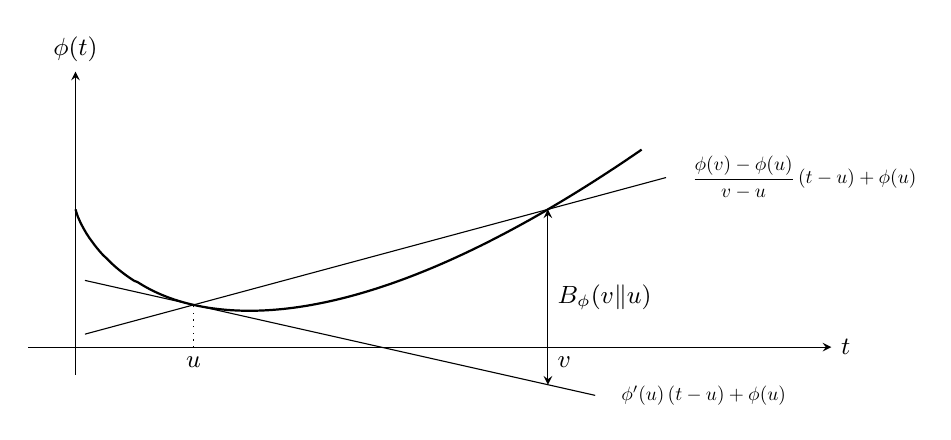
\begin{tikzpicture}
\shorthandoff{>}
%
% Concavidad de - u ln u
\begin{scope}[xscale=6,yscale=3.5]
\pgfmathsetmacro{\u}{.25};
\pgfmathsetmacro{\v}{1};
%
\draw[>=stealth,->] (-.1,-.5)--(1.6,-.5) node[right]{\small $t$};
\draw[>=stealth,->] (0,-.6)--(0,.5) node[above]{\small $\phi(t)$};
\draw[thick,domain=.005:1.2,samples=200] (0,0)-- plot (\x,{\x*ln(\x)});
\draw[dotted] (\u,-.5) node[below]{\small $u$} -- (\u,{\u*ln(\u)});
%\draw[dotted] (\v,-.55) node[below]{\small $v$} -- (\v,{\v*ln(\v)});
\draw[>=stealth,<->] (\v,{(1+ln(\u))*(\v-\u)+\u*ln(\u)}) -- (\v,{\v*ln(\v)});
\draw (\v,-.5) node[below right]{\small $v$};
\draw (\v,{.5*((1+ln(\u))*(\v-\u)+\u*ln(\u)+\v*ln(\v))}) 
node[right]{\small $B_\phi(v\|u)$};
%
\draw (.02,{(.02-\u)*(\v*ln(\v)-\u*ln(\u))/(\v-\u)+\u*ln(\u)})
-- (1.25,{(1.25-\u)*(\v*ln(\v)-\u*ln(\u))/(\v-\u)+\u*ln(\u)})
node[right,scale=.7]
{$\displaystyle \quad \frac{\phi(v)-\phi(u)}{v-u} \, (t-u) + \phi(u)$};;
%
\draw (.02,{(1+ln(\u))*(.02-\u)+\u*ln(\u)})--
(1.1,{(1+ln(\u))*(1.1-\u)+\u*ln(\u)})
node[right,scale=.7]{$\quad \phi'(u) \, (t-u) + \phi(u)$};
\end{scope}
%
%
% % Concavidad / mezcla
% \begin{scope}[xshift=8.5cm]
% \draw(0,1.25) node{\includegraphics[width=3cm]{TIKZ_SZ/DosDados}};
% \draw(-.5,2.5) node{\small $p_1$};
% \draw(1,2) node{\small $p_2$};
% \draw(2.7,1) node{\small $\lambda p_1 + (1-\lambda) p_2$};
% \draw(-.25,-1) node{\includegraphics[width=1cm]{TIKZ_SZ/Moneda}};
% \draw[>=stealth,->,thick] (-.3,-.35)--(-.75,.45);
% \draw (-.525,0) node[left]{\small $\lambda$};
% \draw[>=stealth,->,thick] (-.2,-.35)--(.3,.45);
% \draw (.05,0) node[right]{\small $1-\lambda$};
% \end{scope}
% %
% \draw (1.25,-2.25) node{(a)};
% \draw (8.25,-2.25) node{(b)};
\end{tikzpicture} \end{center}
  %
  \leyenda{$\phi$   convexa:   la    variaci\'on   (cuerda)   $\frac{\phi(v)   -
      \phi(u)}{v-u}$  es  mayor que  la  derivada  $\phi'(u)$.   Aplicado a  dos
    distribuciones $p$ y $q$, de componentes $p_i$ y $q_i$, con $u = p_i$ y $v =
    q_i$  y  sumando, se  obtiene  $\hphi{q}  -  \hphi{p} \ge  \sum_i  (p_i-q_i)
    \phi'(p_i)$ con $H_\phi \equiv H_{(\id,\phi)}, \: \id$ siendo la identidad.}
  %
  \label{fig:SZ:ConvexidadDerivada}
  \end{figure}
  
  Aplicamos esta desigualdad a \ $u = p_{X,Y}(x,y)$ \ y \ $v = p_X(x)
  p_Y(y)$ \ y sumamos en  $x, y$, \ para \ $(a,b) \in ( 0  \, , \, 1)^2$ \ (para
  que  $C_{a,\alpha,b,\beta}$  \ no  sea  reducido  a \  $\{0\}$),  y  \ $c  \in
  \mathring{C}_{a,\alpha,b,\beta}$  \  donde \  $\mathring{\cdot}$  \ denota  el
  interior de un conjunto, se obtiene para $\phi$ convexa,
  %
  \[
  \hphi{p_X \otimes p_Y} - \hphi{p_{X,Y}} \: \le \: c \: g(a,\alpha,b,\beta,c),
  \]
  %
  (para $\phi$  concava se  remplaza $H_\phi$ por  $-H_{-\phi}$ con  la igualdad
  inversa), donde
  %
  \begin{equation}
  g(a , \alpha , b , \beta , c) = \phi'\big( a b + c \big) + \phi'\big( \alpha
  \beta + c \big) - \phi'\big( a \beta - c \big) - \phi'\big( \alpha b - c \big).
  \end{equation}
  %
  Si existe \ $(s,u,t,v) \in \mathring{D}$  \ tal que \ $g(s,u,t,v,0) \ne 0$. De
  la continuidad de $\phi'$, la funci\'on  $g$ es continua, y entonces exista un
  vecinaje  \ $V_0  \subset \mathring{C}_{s,u,t,v}$  \  de \  $0$ \  tal que  la
  funci\'on  \ $c  \mapsto  g(x,u,y,v,c)$ \  tiene  un signo  constante sobre  \
  $V_0$. \ Eso permite  concluir que \ $c \mapsto c \,  g(x,u,y,v,c)$ \ no tiene
  un  signo constante  sobre  \ $V_0$,  \ y  entonces  de concluire  que, de  la
  desigualdad  dedibo   a  la  concavidad  de  $\phi$   (resp.   convexidad),  \
  $\hphi{p_{X,Y}}$ puede ser major  (resp.  menor) que $\hphi{p_X \otimes p_Y}$,
  y   entonces,  con   la  crecencia   (resp.   decrecencia)   de  $h$   que  si
  $g(a,\alpha,b,\beta,0)$  no   es  identicamente  cero   sobre  $\mathring{D}$,
  $H_{(h,\phi)}$ no puede ser subadditiva (conjunta vs product of marginales).

  {\bf Etapa 2}.  Si  $g(a,\alpha,b,\beta,0) = 0$ sobre $\mathring{D}$, entonces
  $\phi'$ satisface la ecuaci\'on funcional
  %
  \[
  \phi'\big( a  b \big)  + \phi'\big(  \alpha \beta \big)  - \phi'\big(  a \beta
  \big) - \phi'\big( \alpha b \big) = 0,
  \]
  %
  as\'i que  no se  puede usar el  argumento de  la etata~1 para  concluir.  Sin
  embargo,     se     puede     solucionar    esta     ecuaci\'on     funcional,
  siguiendo~\cite[\S~6]{DarJar79} donde una  ecuaci\'on funcional muy similar es
  estudiada.  Por  eso, se fija \  $(a,b) \in (0 \,  , \, 1)^2$, \  se deriva la
  identidad precediente  con respeto a \  $\alpha$ \ se  multiplica el resultado
  por $\alpha$ \ para obtener
  %
  \[
  \alpha \beta  \, \phi''(\alpha  \beta) = \alpha  b \, \phi''(\alpha  b) \qquad
  \mbox{for} \qquad (\alpha,\beta) \in (0 \, , \, 1-a) \times (0 \, , \, 1-b).
  \]
  %
  Eso significa  de que $x \,  \phi''(x)$ es constante sobre  $x \in (0  \, , \,
  (1-a)  \max\{b,1-b\})$, y  para cualquier  par $(a,b)  \in (0  \, ,  \, 1)^2$.
  Entonces, $x \, \phi''(x)$ es constante sobre $x \in (0 \, , \, 1 )$, es decir
  que $\phi$ es necesariamente de la forma $\phi(x) = \lambda \, x \ln x + \mu x
  + \nu$. Debido  a la continuidad de $\phi$, queda valide  sobre el cerrado $[0
  \, , \, 1]$.  De que se aplica  a un vector de probabilidad, sumando a uno, se
  puede reducir el problema a $\mu =  0$ (poniendo $\mu$ en $\nu$ sin cambiar el
  valor  de entropia).   Ademas,  la  constante $\nu$  no  altera la  concavidad
  (resp. convexidad) de $\phi$, as\'i que se la puede translatar en la funci\'on
  $h$   (sin  cambiar   la  monotonicidad).    Para  que   $\phi$   sea  convexa
  (resp. concava)  hace falta tener $\lambda  > 0$ (resp.  $\lambda  < 0$) as\'i
  que,  sin perdida  de generalidad,  $\lambda$  puede ser  puesta tambi\'en  en
  $h$. Tomar \ $\phi (x) = x \, \ln x$ \ con \ $h$ \ creciente o \ $\phi (x) = -
  x \, \ln x$ \ con \  $h$ ��� decreciente es completamente equivalente, as\'i que
  se puede fijar $\phi (x) =  x \, \ln x$ satisfaciendo la ecuaci\'on funcional,
  y $h$ creciente.

  $\H_\phi  =   H$  siendo  subadditiva  (propidad~\ref{prop:SZ:subaditividad}),
  cualquier funci\'on creciente de $H$  va obviamente quedar subadditiva, lo que
  cierra la prueba.
  %
\end{proof}
%
Al rev\'es, a partir de $p_{XY}  = \frac12 \begin{bmatrix} 1 & 0 \end{bmatrix}^t
\otimes\begin{bmatrix}  1 &  0  \end{bmatrix}^t +  \frac12  \begin{bmatrix} 0  &
  1  \end{bmatrix}^t \otimes\begin{bmatrix}  0 &  1 \end{bmatrix}^t$  se obtiene
$p_X = p_Y =  \frac12 \begin{bmatrix} 1 & 1 \end{bmatrix}^t$ \  y entonces \ (i)
$\hhphi{p_{XY}}  =  h\left(  -  2  \, \phi\left(  \frac12  \right)  \right)$,  \
$\hhphi{p_X \otimes p_Y} = h\left( -  4 \, \phi\left( \frac14 \right) \right)$ \
y \ $\hhphi{p_X} + \hhphi{p_Y} = 2  \, h\left( - 2 \, \phi\left( \frac12 \right)
\right)$, \  as\'i que, en este  ejemplo \ $\hhphi{p_{XY}}  > \hhphi{p_X \otimes
  p_Y}$  \   (consecuencia  de  la  Schur-convavidad)  y   \  $\hhphi{p_{XY}}  >
\hhphi{p_X}   +   \hhphi{p_Y}$:   Tampoco   las   $(h,\phi)$-entropia   no   son
super-additivas.

\

La  definici\'on  de entropias  generalizadas  condicionales  aparece mucho  mas
problematico. Por  ejemplo, si  se define  a la Shannon,  es decir  definiendo \
$H_{(h,\phi)}(X|Y)$  \  tomando \  $\sum_{y  \in  \Y} p_Y(y)  H_{(h,\phi)}\left(
  p_{X|Y}(\cdot,y)     \right)$     \      se     pierde     la     regla     de
cadena~\ref{prop:SZ:cadena}. Como se lo ha visto,  en el marco de la entropia de
Havdra-Charv\'at-Dar\'oczy, se conserva la regla  de cadena si se remplaza $p_Y$
por su potencia  $p_Y^\beta$.  Sin embargo, generalizar este  esquema en el caso
general falla (la gracia en  Havdra-Charv\'at-Dar\'oczy viene de la propiedad de
morfismo de la  exponencial y del logaritmo). Como  consecuencia, generalizar la
noci\'on se vuelve problematico tambi\'en.  Por ejemple se pierde el diagrama de
Venn  aparte si  se  define la  entropia condicional  a  partir de  la regla  de
cadena. Pero en este caso, si la superadditividad garantiza la positividad de la
entropia             condicional,            se             pierde            la
propiedad~\ref{prop:SZ:independenciacondicional} por  perdida de la additividad,
y          por           consecuencia          la          propiedad          de
positividad/independencia~\ref{prop:SZ:Ipositive}  de  una  informaci\'on  mutua
construida sobre un  modelo diagrama de Venn. Veremos  en la secci\'on siguiente
que  un  tercero  camino  puede  ser usar  divergencia.   \SZ{ver  con  detalles
  \ref{prop:SZ:condicionar} (condiconar)}
%\SZ{VajVas85 pour la Schur-concavite}


\SZ{versiones diferenciales y ver \ref{prop:SZ:biyeccionC} (biyeccion), \ref{prop:SZ:permutacionC} (invarianza por rearreglo~\cite{toto})}

% ================================= Csiszar & Bregman

\subseccion{Divergencias y propiedades}
\label{sec:SZ:Czizar}

\SZ{ (1) Extension a la Renyi, (2) a  la HC/D/T, Cressie Reads, Cressie Pardo, Vajda;
(3) cf Burbea Rao:  (4) generalization Czizar Vajda, et voir avec h phi  avant meme Salicru. Cf
aussi  Bregmann, autres  de Csizsar  2012  versikon Bregman;  gupta Sharma  1976
BoeLub79, Vajda72, Salicru94 Orsak et  Paris; application a le test d'adequation
Pardo 99; MenMor97:5, Cf Pardo 2006 et ref.}

\SZ{FriSri08 pour Bregman; reapparition Fisher comme courbure, cf Varma, Jizba, MenMor97...}


% ================================= Identidades

\subseccion{?`Como se generalizan las identidades y desigualdades?}

\paragraph{Principio de entropia m\'axima} Si este principio naci\'o en el marco de la termodynamica o f\'isica, con la entropia de Shannon (Boltzman), tratando de las nociones generalizadas de incertas, vuelve natural preguntarse sobre la extensi\'on de este problema en el marco general. \SZ{Tal estudio fue hecho en varios trabajos~\cite{ref}  nous, Kesavan,  Kagan 63}.

El problema  se formaliza  como en el caso Shannon,   buscando  la entropia
m\'axima sujeto  a vinculos: sea $X$ variable aleatoria viviendo  sobre $\X \subset \Rset^d$ con $K$ momentos
\  $\Esp\left[ M_k(X)  \right]  = m_k$  \ fijos,  con  $M_x: \X  \to \Rset$,  el
problema  de $(h,phi)$-entropia  m\'axima se  formula de  la manera  siguiente en  el caso
continuo (es el caso discreto, hay que re-emplazar integrales por sumas): sean \
$M(x) = \begin{bmatrix} 1  & M_1(x) & \cdots & M_K(x) \end{bmatrix}^t$  \ y \ $m
= \begin{bmatrix} 1 & m_1 & \cdots & m_K \end{bmatrix}^t$, \ se busca,
%
\[
p^* = \argmax_p \hhphi{p} \qquad \mbox{sujeto a} \qquad p \ge 0, \quad \int_\X M(x)
\, p(x) \, dx = m
\]
%
donde   los  dos  primeros   vinculos  aseguran   de  que   $p^*$  (positividad,
normalizaci\'on) sea  una distribuci\'on de  probabilidad. Si $\phi$  es convexa
(resp.   concava), $h$  es creciente  (resp.  decreciente)  as\'i  que maximizar
$H_{(h,\phi)}$  es equivalente  a maximizar  $H_\phi$ (resp.  $H_{-\phi}$).  Sin
perdida de generalidad, se puede  considerar la situaci\'on $\phi$ convexa. Como
en   el  caso   de  Shannon,   introduciendo  factores   de   Lagrange  $\lambda
= \begin{bmatrix}  \lambda_0 & \lambda_1  & \cdots &  \lambda_K \end{bmatrix}^t$
para  tener  en  cuenta  los   vinculos,  el  problema  variacional  consiste  a
resolver~\cite{GelFom63, Bru04, Mil00, CamMar09, CovTho06}
%
\[
p^* =  \argmax_p \int_\X \left(  - \phi\left( p(x)  \right) + \lambda^t  M(x) \,
  p(x) \right) dx
\]
%
donde $\lambda$ ser\'a  determinado para satisfacer los vinculos.   De nuevo, de
la ecuaci\'on de Euler-Lagrange~\cite{GelFom63,  Bru04} se obtiene la ecuaci\'on
$- \phi'(p(x)) + \lambda^t M(x) = 0$. La funci\'on entropica $\phi$ es concava y
de clase $C^2$, as\'i que $\phi'$ es continua decreciente, y de la monotonicidad
es invertible. Entonces,
%
\[
p^*(x) = \phi'^{-1}\left( \lambda^t M(x) \right)
\]
%
con $\lambda$ tal que se  satisfacen los vinculos de normalizaci\'on y momentos.
Si el resultado no es positivo en  $\X$, de las condiciones KKT, $p^*(x) = \Big(
\phi'^{-1}\left(  \lambda^t M(x)  \right) \Big)_+$.   Estas  distribuci\'ones no
caen  en  general en  la  familia exponencial.  De  una  forma, usando  entropia
generales permite escaparse de esta familia.

Como  en el  caso de  Shannon, queda  obviamente  el hecho  de que  no se  puede
determinar $\lambda$ tal  que se satisfacen todos los  vinculos (y en particular
la de normalizaci\'on).

Tal como en el caso Shannon, existe una prueba informacional:
%
\begin{lema}
  Sea \ $\displaystyle \P_m = \left\{ p \ge 0: \: \int_\X M_k(x) \, p^*(x) \, dx
    =  m \right\}$  \ y  \ $p^*  \in \P_m$  \ que  satisfaga \  $\phi'(p^*(x)) =
  -\lambda^t M(x)$. Entonces
  %
  \[
  \forall  \, p  \in  \P_m,  \quad \hhphi{p}  \le  \hhphi{p^*} \qquad  \mbox{con
    igualdad ssi} \quad p = p^*
  \]
  %
\end{lema}
\begin{proof}
Sin perdida de generalidad, consideramos $\phi$ convexa.
%
\SZ{
\begin{eqnarray*}
\hphi{p} & = & - \int_\X p(x) \, \log p(x) \, dx\\[2.5mm]
%
& = & - \int_\X p(x) \, \log\left( \frac{p(x)}{p^*(x)} \right) \, dx - int_\X
p(x) \, \log p^*(x) \, dx
\end{eqnarray*}
%
De $\log p^* = \lambda^t M$ se obtiene
%
\begin{eqnarray*}
H(p) & = & - D\left( p \left\| p^* \right. \right) - \int_\X \lambda^t M(x) p(x)
\, dx\\[2.5mm]
%
& = & - D\left( p \left\| p^* \right. \right) - \int_\X \lambda^t M(x) \, p^*(x)
\, dx\\[2.5mm]
%
& = & - D\left( p \left\| p^* \right. \right) - \int_\X p^*(x) \log p^*(x) \,
dx\\[2.5mm]
%
& = & - D\left( p \left\| p^* \right. \right) + H(p^*)
\end{eqnarray*}
%
porque $p,  p^* \in \P_m$ \  y \ $\lambda^t M  = \log p^*$. La  prueba se cierra
notando que $D \ge 0$ con igualdad si y solamente si $p = p^*$.
\end{proof}
%
Este lema prueba que, dando  vinculos ``razonables'', la entropia es acotada por
arriba,  y  que  se alcanza  la  cota  para  una  distribuci\'on de  la  familia
exponencial. Por ejemplo,
%
\begin{itemize}
\item Con  $K =  0$ \  y \  $\X$ \ de  volumen finito  \ $|\X|  < +  \infty$, la
  distribuci\'on  de  entropia m\'axima  es  la  distribuci\'on  uniforme de  la
  propiedad~\ref{prop:SZ:cotamaximauniforme}   secci\'on~\ref{sec:SZ:Diferencial}
  en     el      caso     continuo,     o     propiedad~\ref{prop:SZ:cotamaxima}
  secci\'on~\ref{sec:SZ:DefinicionShannon} en el caso discreto.
%
\item Con  $K =  1$, \ $\X  = \Rset^d$  \ y \  $M(x) = x  x^t$ (visto  con $d^2$
  vinculos),  la  distribuci\'on  de  entropia  m\'axima  es  la  distribuci\'on
  gausiana        de        la       propiedad~\ref{prop:SZ:cotamaximagaussiana}
  secci\'on~\ref{sec:SZ:Diferencial}.
\end{itemize}}


\SZ{
   On the theory  of Fisher's
  amount  of  information Sov.  Math.  Dokl., 4  (1963),  pp.  991-993, etc,  la
  codificaci\'on a la Renyi (Cambell,  Hooda 2001, Bercher) 

\

 y la cuantificacion
  fina; EPI generalizada por Madiman, etc. Lutwak, Bercher etc., Kagan; Boeke 77
  An extension  of the Fisher information  measure I. Csisz\'ar,  P. Elias (Eds.),
  Topics   in  Information  Theory,   North-Holland,  Berlin/New   York  (1977),
  pp. 113-123  o Hammad o  Vajda 73 o  Ferentinos81 en el marco  Fisher; Kesavan
  gene MaxEnt}

\SZ{Revisite capacite a la Daroczy? codage; parler de la quantification fine et HCD}
